\documentclass[10pt, compress]{beamer}

\usetheme[numbering=fraction, sectionpage=none, progressbar=frametitle]{m}
\usepackage{booktabs}
\usepackage{array}
\usepackage{listings}
\usepackage{graphicx}
\usepackage[portuguese]{babel}
\usepackage[scale=2]{ccicons}

\usepackage{url}
\usepackage{relsize}
\usepackage{courier}
\usepackage{tgcursor}

\usepackage{pgfplots}
\usepgfplotslibrary{dateplot}

\lstset{basicstyle=\footnotesize\ttfamily,breaklines=true}
\renewcommand*{\UrlFont}{\ttfamily\smaller\relax}
\renewcommand*{\ttdefault}{qcr}

\graphicspath{{./img/}}

\title{Ajuste Fino Automatizado utilizando Computação em Nuvem}
\subtitle{}
\date{29 de Setembro de 2015}
\author{Pedro Bruel \\ phrb@ime.usp.br}
\institute{Departamento de Ciência da Computação do IME, USP \\ MAC5910 - Programação para Redes de Computadores}
\titlegraphic{\hfill
\includegraphics[height=2cm]{imelogo}}

\begin{document}

\maketitle

\section{Motivações}

\begin{frame}[fragile]
  \frametitle{Motivações}
  \begin{figure}[H]
      \centering
      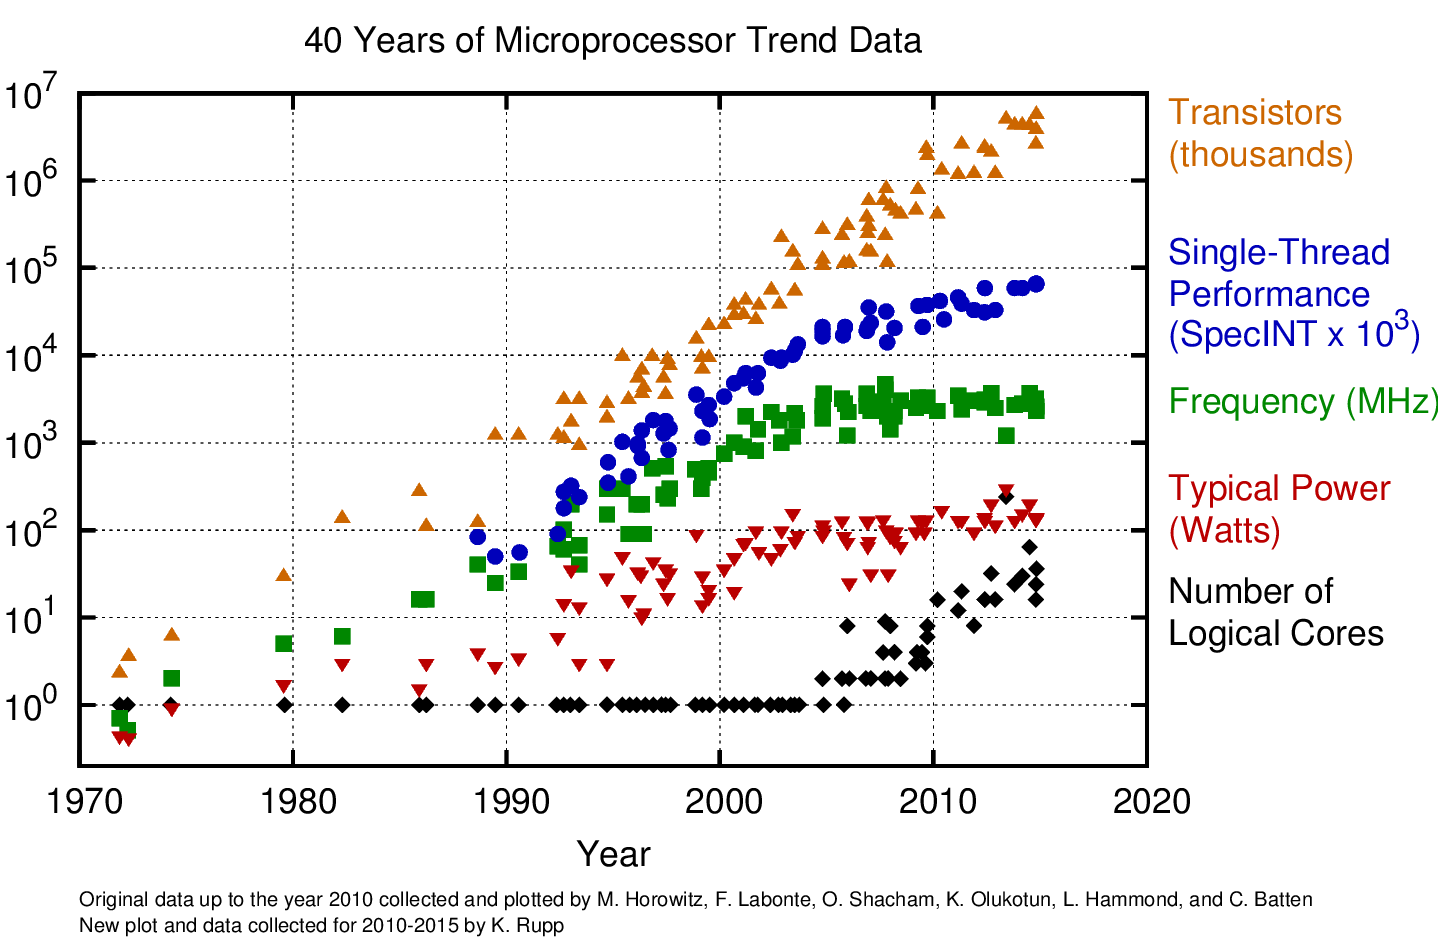
\includegraphics[width=1\textwidth]{40years}
  \end{figure}
    \let\thefootnote\relax\footnotetext{\url{http://karlrupp.net/2015/06/40-years-of-microprocessor-trend-data}}
\end{frame}

\begin{frame}[fragile]
  \frametitle{Uma Solução: \emph{Autotuning}}
  \begin{columns}
      \column{0.5\textwidth}
      \centering
      Configurações e Otimizações
      \column{0.5\textwidth}
      \centering
      Espaço de Busca
  \end{columns}
  \begin{figure}[H]
      \centering
      \includegraphics[width=1\textwidth]{autotuning}
  \end{figure}
\end{frame}

\begin{frame}[fragile]
  \frametitle{\emph{Autotuning}: OpenTuner}
  \begin{figure}[H]
      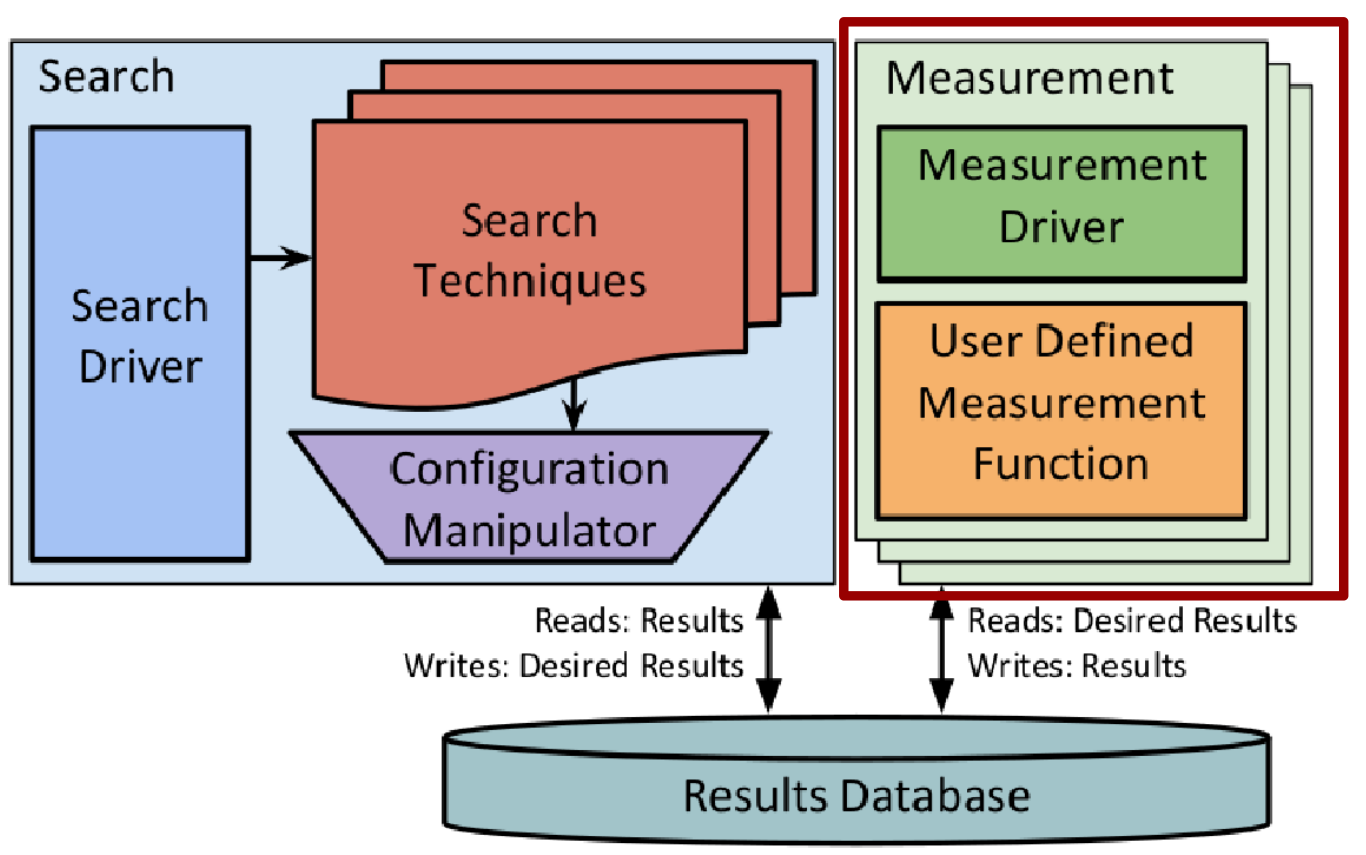
\includegraphics[width=0.65\textwidth]{opentuner-measurement.png}
  \end{figure}
  Medições são sempre feitas \alert{localmente} e \alert{sequencialmente}
  \footnotetext[2]{Imagem: Ansel, Jason, et al. "Opentuner: An extensible framework for program autotuning." Proceedings of the 23rd ICPAC. ACM, 2014.}
\end{frame}

\section{Objetivos}

\begin{frame}[fragile]
  \frametitle{Objetivos}
  \alert{Modificar} o arcabouço OpenTuner para que seja possível
  realizar medições \alert{distribuídas} na nuvem

  \alert{RQ1}: Como normalizar medições de desempenho feitas na nuvem?

  \alert{RQ2}: Para que tipo de problema é vantajoso utilizar os recursos da nuvem?
\end{frame}

\begin{frame}[fragile]
  \frametitle{Objetivos: Lista}
  \alert{DONE}:
  \begin{itemize}
      \item \alert{MeasurementClient}
      \item \alert{MeasurementServer}
      \item \alert{Interface} com a Google Compute Engine
      \item \alert{Protocolo} de Aplicação
      \item Avaliação de \alert{desempenho} para o \alert{TSP},
          em alguns casos
      \item Correção de um \alert{bug} no OpenTuner: 
          \url{https://github.com/jansel/opentuner/pull/73}
  \end{itemize}
  \alert{TODO}:
  \begin{itemize}
      \item \alert{Normalização} de Resultados
      \item Composição do \alert{benchmark}
      \item Avaliação de \alert{desempenho} em mais problemas
          e casos
  \end{itemize}
\end{frame}

\section{Implementação}

\begin{frame}[fragile]
  \frametitle{Usando a Google Compute Engine}
  \begin{itemize}
      \item Período de \alert{trial}: US\$300 por 60 dias 
      \item Usei as máquinas de \alert{menor desempenho}: apenas uma CPU
      \item Número limitados de \alert{CPUs} e \alert{IPs} por região: 23
      \item Construí uma \alert{imagem} para \alert{acelerar a inicialização} das VMs
      \item \alert{Dificuldades} com os experimentos
  \end{itemize}
\end{frame}

\begin{frame}[fragile]
  \frametitle{Cliente e Servidor}
    \begin{columns}
        \column{0.5\textwidth}
        \begin{figure}[H]
            \centering
            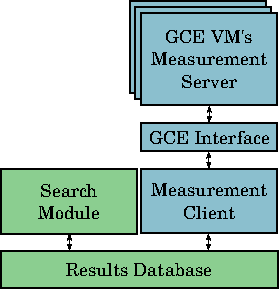
\includegraphics[scale=.62]{high-level-implementation}
        \end{figure}%
        \column{0.5\textwidth}
        \begin{figure}[H]
            \centering
            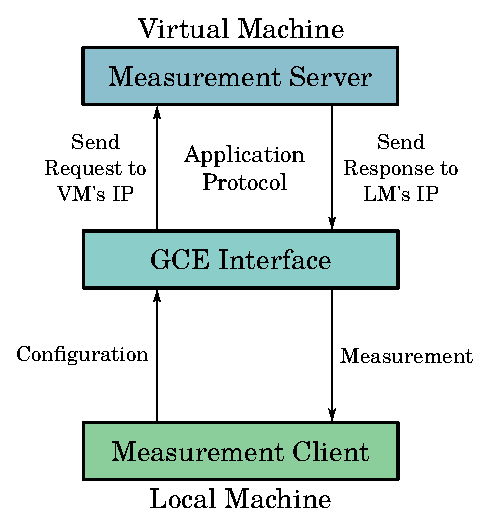
\includegraphics[scale=.62]{low-level-implementation}
        \end{figure}%
    \end{columns}
\end{frame}

\begin{frame}[fragile]
  \frametitle{OpenTuner: Fluxo de Execução}
  \begin{figure}[H]
      \centering
      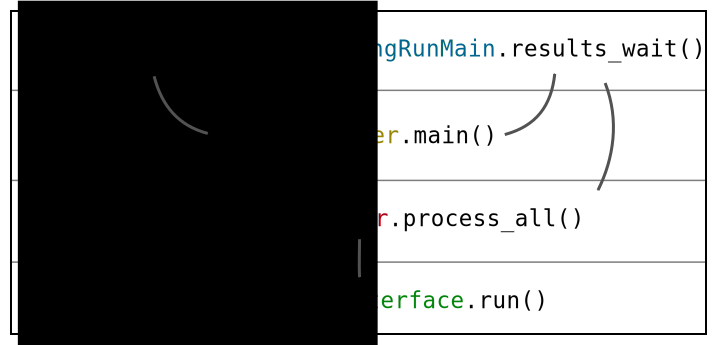
\includegraphics[width=.8\textwidth]{opentunerflow_simple}
  \end{figure}
\end{frame}

\begin{frame}[fragile]
  \frametitle{Esforço de Implementação}
  \begin{figure}[H]
      \centering
      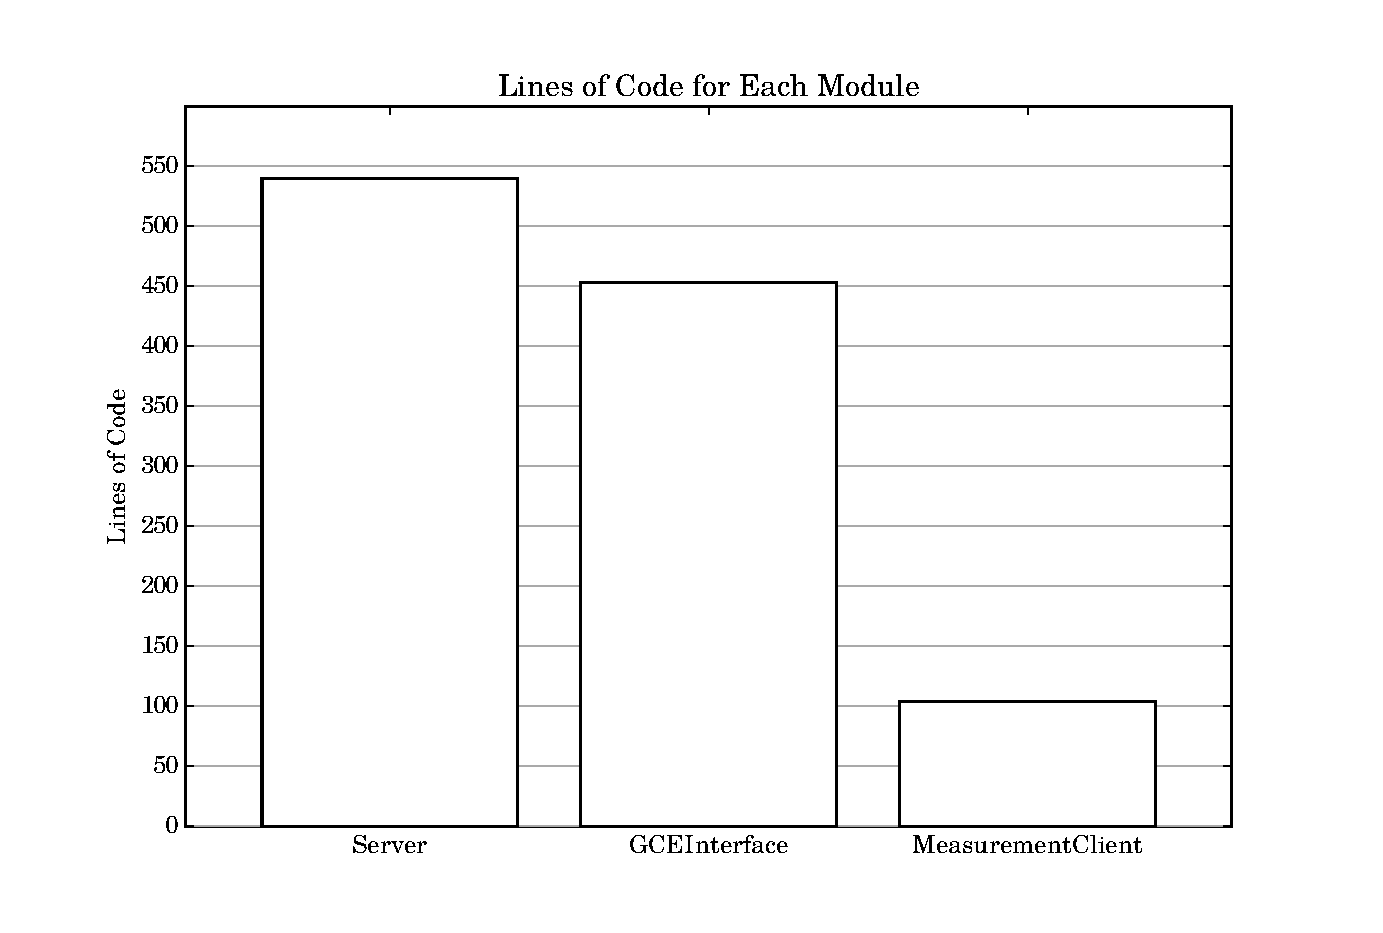
\includegraphics[width=1\textwidth]{loc_comparison}
  \end{figure}
\end{frame}

\begin{frame}[fragile]
    \frametitle{Servidor}
    Disponível sob GPL em:
    \url{https://github.com/phrb/measurement-server}
    \begin{itemize}
        \item Executado nas \alert{máquinas virtuais}
        \item Espera por uma \alert{conexão} TCP na porta 8080
        \item Espera por \alert{comandos}
        \item \alert{Obtém} o projeto do usuário à partir
            de um \alert{repositório git}
        \item \alert{Importa a classe} do usuário no servidor
        \item \alert{Executa medições} utilizando o método
            \texttt{run} do usuário
    \end{itemize}
\end{frame}

\begin{frame}[fragile]
  \frametitle{Protocolo: Mensagens}
  \newcolumntype{K}{>{\centering\arraybackslash}m{5cm}}
\newcommand{\specialcell}[2][c]{%
  \begin{tabular}[#1]{@{}K@{}}#2\end{tabular}}

\newcolumntype{T}{>{\centering\arraybackslash}m{1.5cm}}
\newcolumntype{L}{>{\centering\arraybackslash}m{2.4cm}}

\begin{table}[htpb]
    \centering
    \tiny
    \begin{tabular}{@{}TLK@{}}
        \toprule
        {\bf Command} & {\bf Function} & {\bf Message} \\ \midrule
        {\tiny \bf START} & 
        {\tiny Sets the server's status to AVAILABLE} & 
        {\tiny \tt ``START''} \\ \midrule
        {\tiny \bf STOP} & 
        {\tiny Sets the server's status to STOPPED} & 
        {\tiny \tt ``STOP''} \\ \midrule
        {\tiny \bf STATUS} & 
        {\tiny Requests the server current status} & 
        {\tiny \tt ``STATUS''} \\ \midrule
        {\tiny \bf DISCONNECT} & 
        {\tiny Disconnects from the server} & 
        {\tiny \tt ``DISCONNECT''} \\ \midrule
        {\tiny \bf SHUTDOWN} & 
        {\tiny Disconnects and shuts the server down} & 
        {\tiny \tt ``SHUTDOWN''} \\ \midrule
        {\tiny \bf CLONE} & 
        {\tiny Clones a git repository to the virtual machine} & 
        {\tiny \tt ``CLONE REPO\_URL DIST\_DIR''} \\ \midrule
        {\tiny \bf LOAD} & 
        {\tiny Imports the user's MeasurementInterface into the server} & 
        {\tiny \tt ``LOAD TUNER\_PATH INTERFACE\_NAME''} \\ \midrule
        {\tiny \bf MEASURE} & 
        {\tiny Computes the measurement for a given configuration} & 
        {\tiny \tt ``MEASURE CONFIG INPUT LIMIT''} \\ \midrule
        {\tiny \bf GET} & 
        {\tiny Requests a configuration's result} & 
        {\tiny \tt ``GET RESULT\_ID''} \\ \bottomrule
    \end{tabular}
    \caption{Server messages.}
    \label{tab:protocol-messages}
\end{table}

\end{frame}

\begin{frame}[fragile]
  \frametitle{Protocolo: Respostas}
  \newcolumntype{K}{>{\centering\arraybackslash}m{8.2cm}}
\newcommand{\specialcell}[2][c]{%
  \begin{tabular}[#1]{@{}K@{}}#2\end{tabular}}

\newcolumntype{T}{>{\centering\arraybackslash}m{1.5cm}}

\begin{table}[htpb]
    \centering
    \tiny
    \begin{tabular}{@{}TK@{}}
        \toprule
        {\bf Received Command} & {\bf Response} \\ \midrule
        {\tiny \bf START} &
        {\tiny \tt ``START ERROR\_STATUS SERVER\_STATUS''} \\ \midrule
        {\tiny \bf STOP} &
        {\tiny \tt ``STOP ERROR\_STATUS SERVER\_STATUS''} \\ \midrule
        {\tiny \bf STATUS} &
        {\tiny \tt ``STATUS ERROR\_STATUS SERVER\_STATUS''} \\ \midrule
        {\tiny \bf DISCONNECT} &
        {\tiny \tt ``DISCONNECT ERROR\_STATUS SERVER\_STATUS''} \\ \midrule
        {\tiny \bf SHUTDOWN} &
        {\tiny \tt ``SHUTDOWN ERROR\_STATUS SERVER\_STATUS''} \\ \midrule
        {\tiny \bf CLONE} &
        {\tiny \tt ``CLONE ERROR\_STATUS SERVER\_STATUS [GIT\_RET\_CODE]''} \\ \midrule
        {\tiny \bf LOAD} &
        {\tiny \tt ``LOAD ERROR\_STATUS SERVER\_STATUS''} \\ \midrule
        {\tiny \bf MEASURE} &
        {\tiny \tt ``MEASURE ERROR\_STATUS SERVER\_STATUS [RESULT\_ID]''} \\ \midrule
        {\tiny \bf GET} &
        {\tiny \tt ``GET ERROR\_STATUS SERVER\_STATUS [RESULT\_ID] [RESULT]''} \\ \bottomrule
    \end{tabular}
    \caption{Server responses.}
    \label{tab:protocol-responses}
\end{table}

\end{frame}

\begin{frame}[fragile]
  \frametitle{Protocolo: Respostas Numéricas}
  \newcolumntype{K}{>{\centering\arraybackslash}m{2.8cm}}
\newcommand{\specialcell}[2][c]{%
  \begin{tabular}[#1]{@{}K@{}}#2\end{tabular}}

\newcolumntype{T}{>{\centering\arraybackslash}m{.3cm}}
\newcolumntype{L}{>{\centering\arraybackslash}m{4cm}}

\begin{table}[htpb]
    \centering
    \tiny
    \begin{tabular}{@{}KTL@{}}
        \toprule
        {\bf Response} & {\bf Code} & {\bf Meaning} \\ \midrule
        {\tiny \bf NO\_ERROR} & 
        {\tiny \tt 0} & 
        {\tiny No errors occurred} \\ \midrule
        {\tiny \bf AVAILABLE} & 
        {\tiny \tt 1} & 
        {\tiny Server state: The server is waiting for messages} \\ \midrule
        {\tiny \bf STOPPED} & 
        {\tiny \tt 2} & 
        {\tiny Server state: The server is not running} \\ \midrule
        {\tiny \bf UNAVAILABLE\_ERROR} & 
        {\tiny \tt 3} & 
        {\tiny The server was not available} \\ \midrule
        {\tiny \bf UNKNOWN\_COMMAND\_ERROR} & 
        {\tiny \tt 4} & 
        {\tiny Received an unknown command} \\ \midrule
        {\tiny \bf ARGUMENT\_ERROR} & 
        {\tiny \tt 5} & 
        {\tiny Wrong number of arguments} \\ \midrule
        {\tiny \bf GITCLONE\_ERROR} & 
        {\tiny \tt 6} & 
        {\tiny Error cloning repository} \\ \midrule
        {\tiny \bf NO\_FILE\_ERROR} & 
        {\tiny \tt 7} & 
        {\tiny Couldn't find user classes} \\ \midrule
        {\tiny \bf NO\_RUN\_METHOD\_ERROR} & 
        {\tiny \tt 8} & 
        {\tiny Couldn't find run method} \\ \midrule
        {\tiny \bf STARTED\_ERROR} & 
        {\tiny \tt 9} & 
        {\tiny The server was already started} \\ \midrule
        {\tiny \bf NOT\_READY\_ERROR} & 
        {\tiny \tt 10} & 
        {\tiny The server was not started} \\ \midrule
        {\tiny \bf NO\_SUCH\_RESULT\_ERROR} & 
        {\tiny \tt 11} & 
        {\tiny The requested result is not on this machine} \\ \bottomrule
    \end{tabular}
    \caption{Numeric responses.}
    \label{tab:protocol-errors}
\end{table}

\end{frame}

\begin{frame}[fragile]
    \frametitle{Interface}
    Disponível sob GPL em:
    \url{https://github.com/phrb/gce_interface}
    \begin{itemize}
        \item \alert{Encapsula} a comunicação com o servidor
        \item \alert{Serializa e deserializa} os resultados e requisições
            usando o módulo \alert{pickle} do Python
        \item \alert{Coordena} a inicialização e término das máquinas
            virtuais
    \end{itemize}
\end{frame}

\begin{frame}[fragile]
    \frametitle{Cliente}
    Disponível sob GPL em:
    \url{https://github.com/phrb/measurement_client}
    \begin{itemize}
        \item \alert{Processa} requisições de 
            resultados do OpenTuner
        \item \alert{Executa} código do Usuário
        \item Faz \alert{requisições} de resultados à interface
    \end{itemize}
\end{frame}

\begin{frame}[fragile]
  \frametitle{Fluxo de Execução}
  \begin{figure}[H]
      \centering
      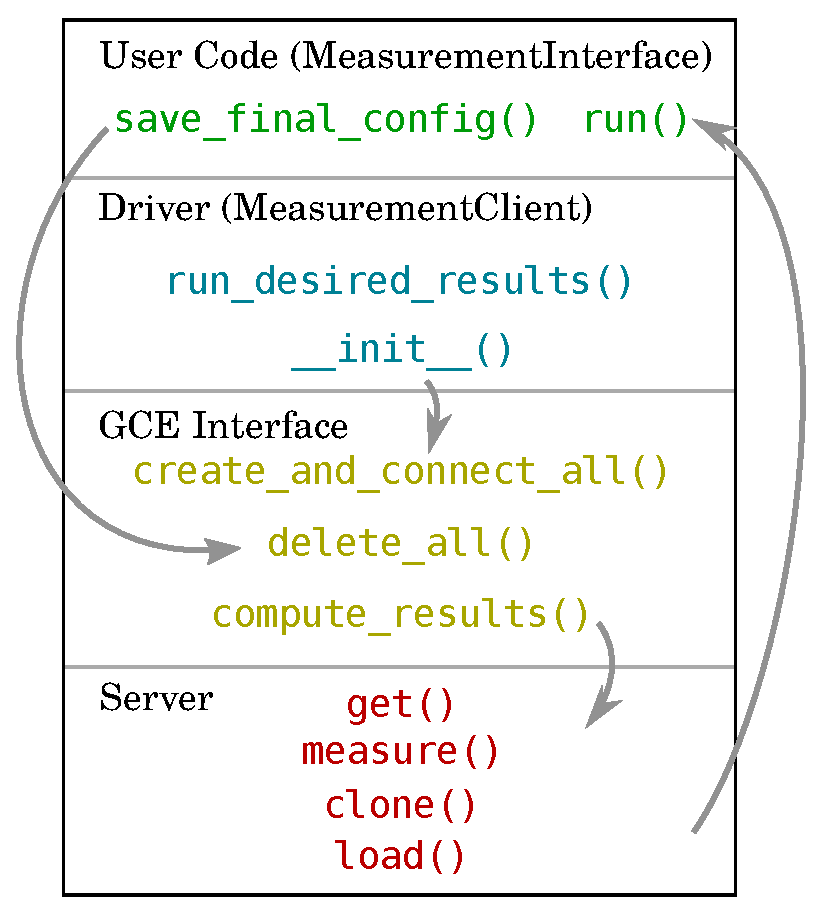
\includegraphics[width=.5\textwidth]{interfaceflow_simple}
  \end{figure}
\end{frame}

\section{Resultados Parciais}

\begin{frame}[fragile]
    \frametitle{Experimentos: Travelling Salesperson Problem}
    \begin{figure}[H]
        \centering
        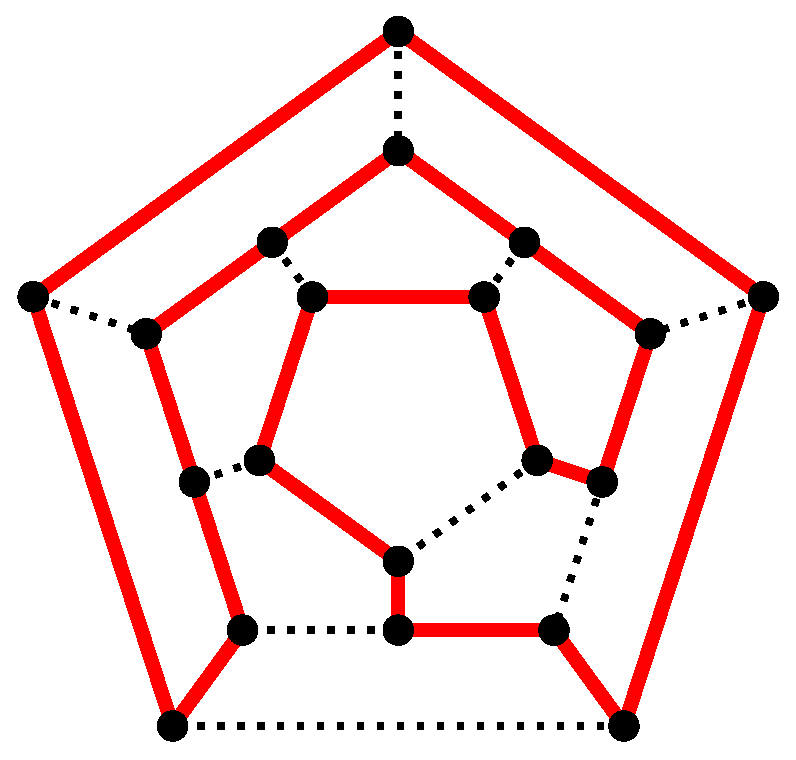
\includegraphics[width=.33\textwidth]{hamiltonianpath}
    \end{figure}%
    Encontrar o \alert{menor caminho} que passa por todos os vértices de um
    grafo, \alert{voltando ao vértice de origem}.

    As soluções são representadas como \alert{permutações} de cidades.

    \alert{Avaliação do desempenho} de um resolvedor de
    instâncias do TSP implementados com o OpenTuner. 

    Medições com números diferentes de \alert{máquinas virtuais} e de
    \alert{requisições simultâneas}.
\end{frame}

\begin{frame}[fragile]
  \frametitle{TSP: Resultados Parciais}
  \begin{figure}[H]
      \centering
      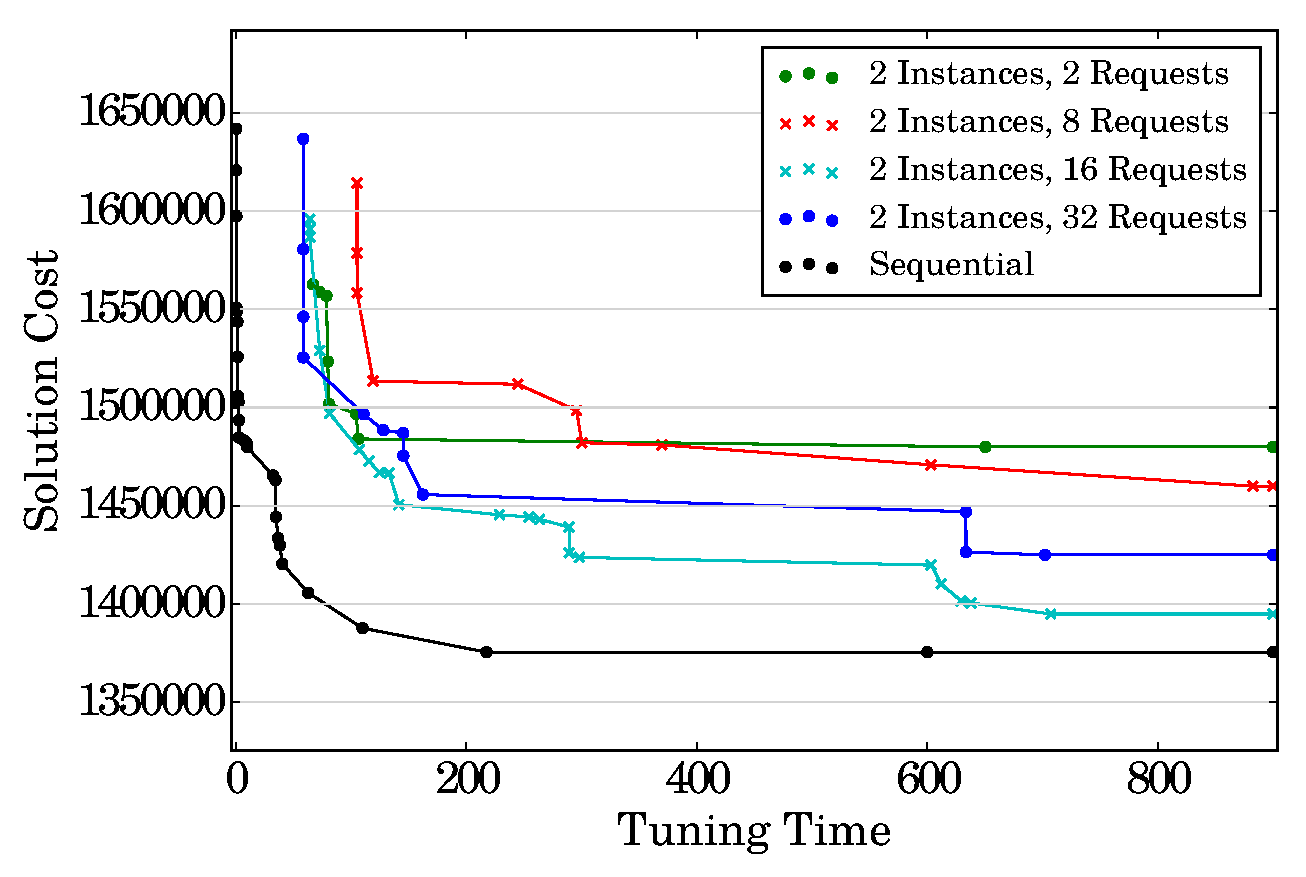
\includegraphics[width=.8\textwidth]{i2_p_n_comparison}
  \end{figure}
\end{frame}

\begin{frame}[fragile]
  \frametitle{TSP: Resultados Parciais}
  \begin{figure}[H]
      \centering
      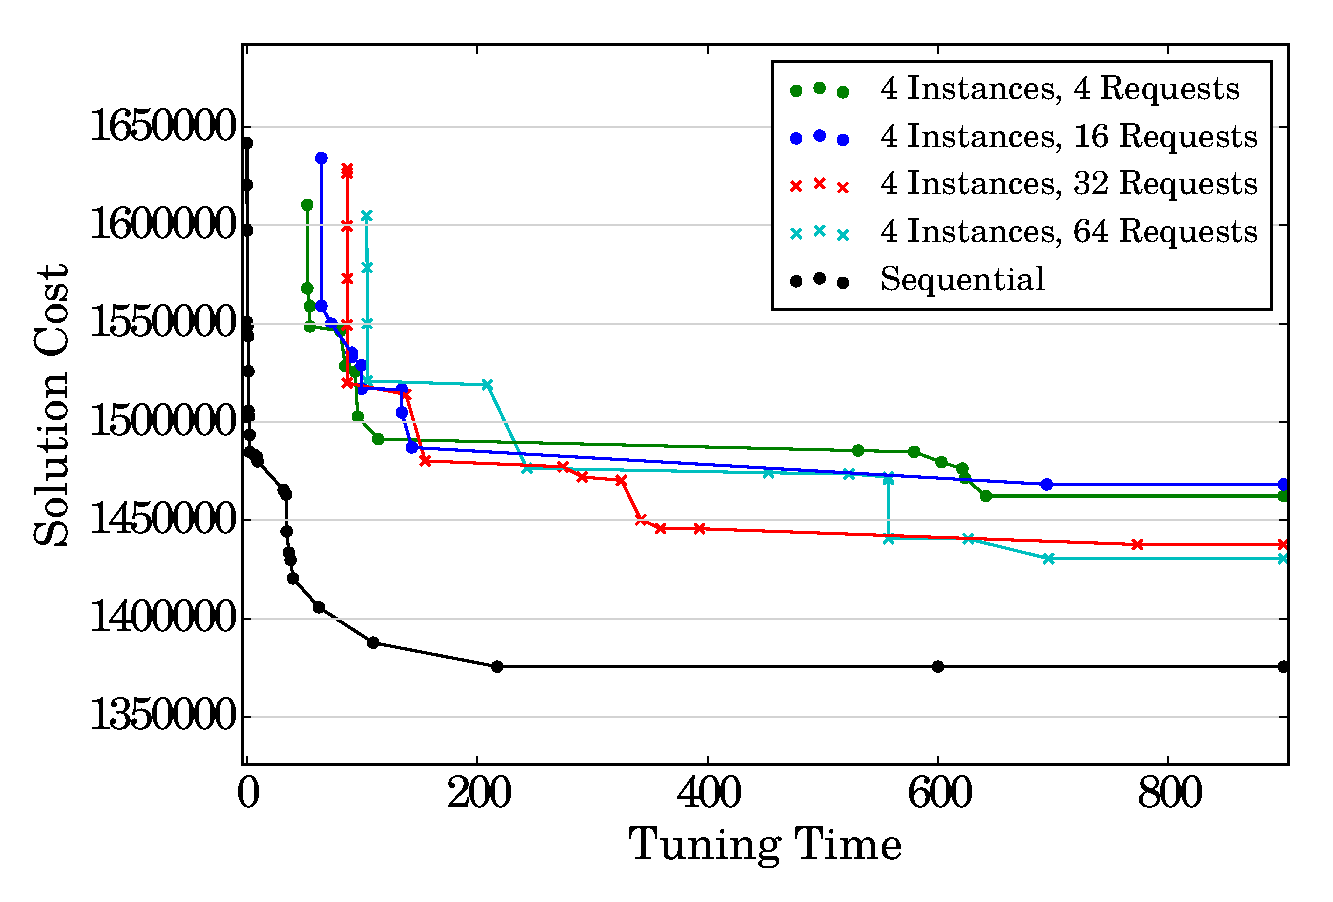
\includegraphics[width=.8\textwidth]{i4_p_n_comparison}
  \end{figure}
\end{frame}

\begin{frame}[fragile]
  \frametitle{Normalização de Resultados}
  \textbf{RQ1}: Como aplicar os resultados obtidos em máquinas virtuais
  \alert{diferentes da máquina local}?

  \begin{itemize}
      \item Autotuning do \alert{modelo de desempenho}
      \item \alert{Combinar} resultados diferentes
      \item \alert{Simular} a máquina local
      \item Executar o autotuner na \alert{nuvem}
  \end{itemize}
\end{frame}

\plain{Obrigado!}

\maketitle

\end{document}
